\documentclass[../../dissertation.tex]{subfiles}
\begin{document}

The design was based on the decomposition of the evolution equation
\begin{equation}
    \ket{\psi(t)} = U(t) \psi(0),
\end{equation}
into several constituent classes, namely a \texttt{State} class composed of a
column array for representing the initial and final state of the walk, an
\texttt{Operator} class for building the Hamiltonian associated with a certain
graph, a \texttt{QuantumWalk} class for combining the operator and the initial
state and outputting the final state, and a \texttt{ProbabilityDistribution}
class for converting amplitudes into probabilities.\par
\begin{figure}[!h]
    \centering
    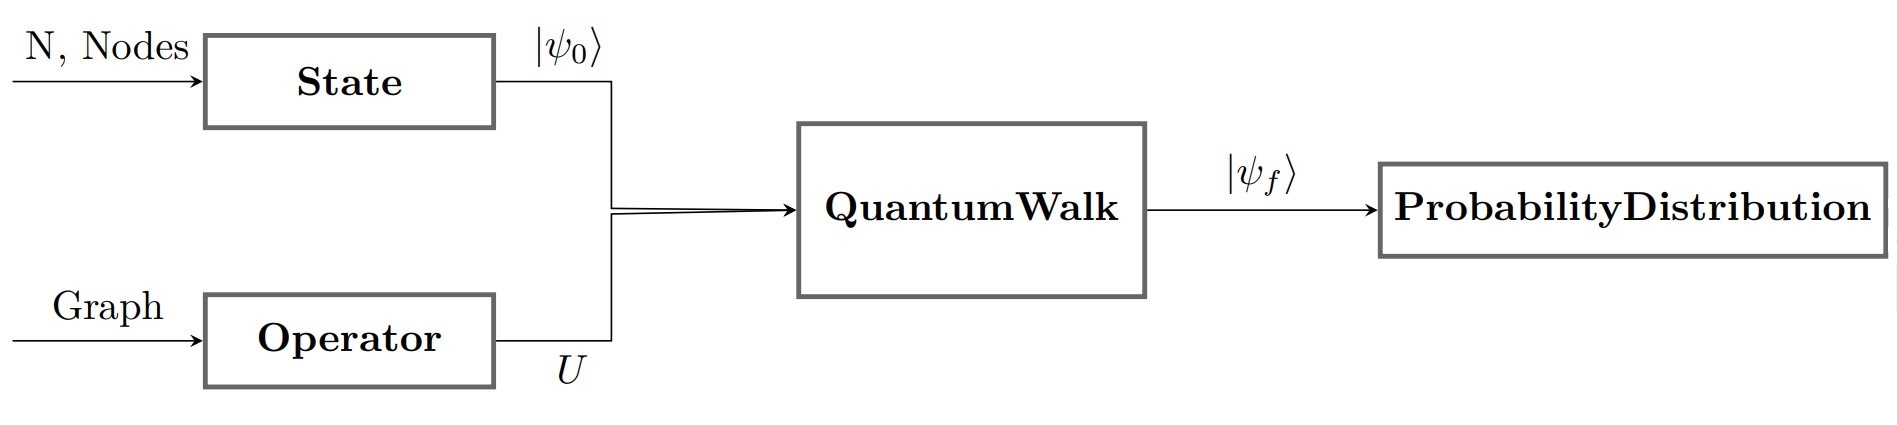
\includegraphics[width=12cm]{img/QWAK/qwakDiagram.jpg}
    \caption{Directed infinite line with weights $e^{i\alpha}$ and $e^{-i\alpha}$.}
    \label{fig:oriented_line}
\end{figure}

Finally, the \texttt{QWAK} class combines all of the previous components
providing the user a simplified way of performing and analyzing the CTQW.
Analogously, these classes were also similarly defined for the stochastic
quantum walk case, except for the \texttt{State} class. They then culminate in
the \texttt{StochasticQWAK} class which performs a similar role as the
controller but with different inputs and calculation methods. Documentation on
the classes and methods available in this package are available on GitHub pages
\footnote{https://jaimepsantos.github.io/QWAK/}. 

%TODO Adicionar uma tabela com as classes?
%TODO Link para a doc.
%TODO Mencionar Stochastic ou dizer depois que segue a mesma logica?

\subsubsection{State Class}
\begin{lstlisting}[style=commands,language=Python]
    class State(n, nodeList: list = None, customNodeList: list = None)
\end{lstlisting}
This class takes the dimension of the walk \texttt{n} as input and creates a
\texttt{NumPy ndarray} with as many elements. The \text{nodeList} parameter is
a list of integers, and it initializes the \texttt{nodeList} attribute, which
later will be used to create a uniform superposition of the chosen nodes.
Alternatively, the user can choose the amplitudes individually by passing a
list of pairs through the \texttt{customStateList} parameter. If the user
chooses not to set the optional parameters, the attributes will be initialized
as a vector filled with $0$'s. If the resulting custom state is not
unitary, an exception of the \texttt{NonUnitaryState} type will be thrown.
Similarly, passing a node greater than the state's dimension will
raise a \texttt{StateOutOfBounds} exception.\par 

For example, creating the uniform superposition of the state
\begin{equation}
    \ket{\psi} = \frac{1}{\sqrt{4}}\left( \ket{0} + \ket{1} +\ket{2} +\ket{3}\right),
\end{equation}
can be done via the following code:
\begin{lstlisting}[style=code]
    from qwak.State import State

    n = 4
    initNodes = [0,1,2,3]
    initState = State(n,initNodes)
    initState.buildState()
    print(initState.getStateVec())
\end{lstlisting}
producing the subsequent array as output:

\begin{lstlisting}[style=commands,mathescape]
@$>$   [[0.5+0.j] [0.5+0.j] [0.5+0.j] [0.5+0.j]] @
\end{lstlisting}

The \texttt{buildState} function is responsible for creating either the uniform
superposition or custom state, with the following parameters: 
\begin{lstlisting}[style=commands,mathescape,language=Python]
    def buildState(nodeList: list = None, customStateList: list = None)
\end{lstlisting}
The user can define the amplitudes of the nodes either at
initialization or at building time, which will be useful to change the desired
state without creating a new object. The \texttt{getStateVec} function simply
returns the array of the state. The remaining available methods are described
in the documentation. 

\subsubsection{Operator Class}
\begin{lstlisting}[style=commands,mathescape,language=Python]
    class Operator(graph: nx.Graph , laplacian: bool = False, markedSearch: list = None)
\end{lstlisting}
The graph parameter must be a \texttt{NetworkX} graph object initialized with
the correct number of nodes, which will be used to initialize the
\texttt{adjacencyMatrix} attribute. If the \texttt{laplacian} attribute is set
to \texttt{true}, then the Hamiltonian will be built with the Laplacian matrix
instead. The \texttt{markedSearch} parameter is a list of tuples containing
pairs of amplitudes and nodes, which will change the adjacency matrix
accordingly, in order to perform a search using the CTQW.\par

The operator can be constructed via the following procedure:
\begin{lstlisting}[style=code,escapeinside={__}]
    from qwak.Operator import Operator 
    import networkx as nx
    
    t = 2
    graph = nx.cycle_\textunderscore_graph(n)
    operator = Operator(graph)
    operator.buildDiagonalOperator(t)
    print(operator.getOperator())
\end{lstlisting}
resulting in the following matrix as output:
\begin{lstlisting}[style=commands,mathescape]
@$>$
       [[  0.77-0.j    -0.-0.421j   -0.23-0.j   -0.-0.421j  ]
       [  -0.-0.421j    0.77+0.j    -0.-0.421j  -0.23+0.j   ]
       [  -0.23-0.j    -0.-0.421j    0.77-0.j   -0.-0.421j  ]
       [  -0.-0.421j   -0.23+0.j    -0.-0.421j   0.77+0.j   ]] @
\end{lstlisting}

The \texttt{buildDiagonalOperator} method presented an important challenge
regarding the performance of \texttt{QWAK}, and is responsible for the time
evolution: 
\begin{lstlisting}[style=commands,mathescape,language=Python]
    def buildDiagonalOperator(self, time: float = 0)
\end{lstlisting}
\begin{figure}[!h]
	\centering
	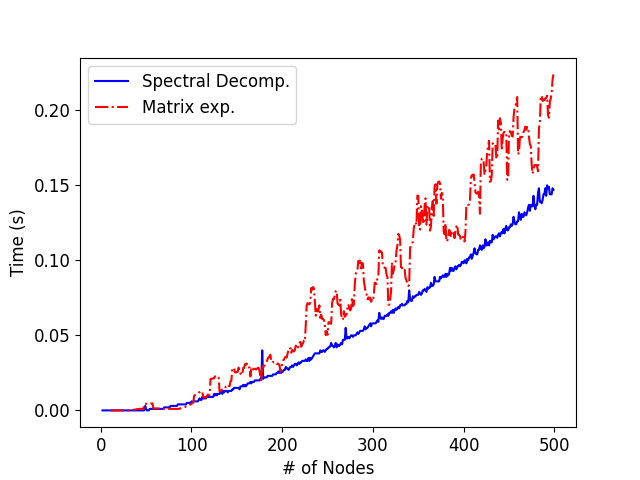
\includegraphics[scale=0.50]{img/QWAK/expmVsDiag.png}
	\caption{Comparison between the execution time of the spectral decomposition and the matrix exponential methods, as a function of the number of nodes.} 
	\label{fig:expmVsDiag}
\end{figure}
The operator of the quantum walk was previously defined in equation
\eqref{eq:contSimulUniOp} as 
\begin{equation} 
    U(t) = \phi(t) e^{i\gamma A t},
\end{equation} where matrix exponentiation is required. This can be achieved
with \texttt{SciPy}'s \texttt{expm} function, with a very significant
computational cost. Alternatively, we calculate the spectral decomposition of
$U$
\begin{equation}
    U = Q e^{i\Lambda t} Q^{-1} ,
\end{equation}
where $Q$ is a matrix containing the eigenvectors of the adjacency matrix, and 
\begin{equation}
    \Lambda = \sum_{j} \lambda_j \ket{j}\bra{j},
\end{equation}
%TODO Escrever e explicar codigo do buildDiagonal?
is a diagonal operator that encodes the eigenvalues. For this effect, we use
\texttt{NumPy}'s linear algebra methods. If the adjacency matrix is
non-hermitian, then the general solution \texttt{eig} is used, otherwise
\texttt{eigh} can be employed at a lower cost. Even though calculating
eigenvectors and eigenvalues is relatively costly, matrix size gets
significantly reduced when dealing with hermitian matrices, resulting in better
performance when compared to \texttt{expm} as seen in figure
\ref{fig:expmVsDiag}.\par
\begin{figure}[!h]
	\centering
	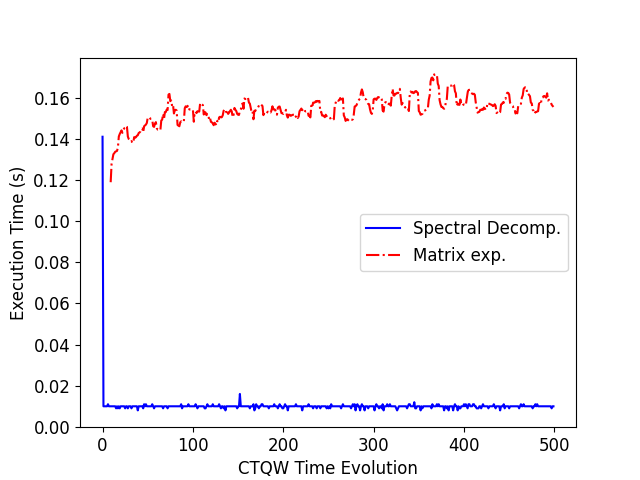
\includegraphics[scale=0.50]{img/QWAK/expmVsDiagTime.png}
    \caption{Comparison between the execution time of the spectral decomposition and the matrix exponential methods, for a fixed number of nodes with varying evolution time.} 
	\label{fig:expmVsDiagTime}
\end{figure}
%TODO: Meter figura do performance vs tempo?
The performance increase is even more significant when creating, for example,
animated evolutions of the probability distribution. For a fixed-size graph,
the eigenvectors and eigenvalues are not affected by a change in the time
evolution, which means that we can set up our \texttt{Operator} implementation
to calculate these quantities at object initialization. We can then run
\texttt{buildDiagonalOperator} for each time value we choose and generate the
corresponding operators at a very low cost. However, the \texttt{expm} implementation
will recalculate everything for each inputted time.
Figure \ref{fig:expmVsDiagTime} shows that the spectral decomposition method
has a relatively high cost for the first iteration of the walk, corresponding
to the use of the \texttt{eigh} function, and then it remains constant and has a much
lower cost than exponentiating the matrix.\par
The \texttt{Operator} class further provides the \texttt{checkPST} method for
determining whether a graph exhibits perfect state transfer between specific 
nodes and calculating the exact time of that transfer in case it does. This
method was implemented based on the work by \cite{coutinho17}. 

\subsubsection{QuantumWalk Class}

\begin{lstlisting}[style=commands,language=Python,mathescape]
    class QuantumWalk(state: State, operator: Operator)
\end{lstlisting}
We can now combine the previously defined initial state with the operator 
to obtain the evolution's final state. We delegate this to the
\texttt{QuantumWalk} class, and it can be straightforwardly used as follows:
\begin{lstlisting}[style=code,escapeinside={__}]
    from qwak.QuantumWalk import QuantumWalk 

    quantumWalk = QuantumWalk(initState,operator)
    quantumWalk.buildWalk()
    finalState = quantumWalk.getFinalState()
    print(finalState.getStateVec())
\end{lstlisting}
and it produces a column array as output:
\begin{lstlisting}[style=commands,mathescape]
@$>$ [[0.27-0.421j] [0.27-0.421j] [0.27-0.421j] [0.27-0.421j]]
\end{lstlisting}\par

The final state is achieved through the \texttt{buildWalk} method: 
\begin{lstlisting}[style=commands,mathescape,language=Python]
    def buildWalk(self, initState: State = None, operator: Operator = None)
\end{lstlisting}
which multiplies the operator matrix by the state array and sets the
\texttt{finalState} attribute to the resulting amplitudes. We can then access
this \texttt{State} object via the \texttt{getFinalState} method, and the
%TODO InvPartRatio, SurvProb  : Aperiodic space-inhomogeneous quantum walks:
%localization properties, energy spectra and enhancement of entanglement
%Graphs
associated \texttt{ndarray} with \texttt{getStateVec}. The class further
provides methods for calculating certain transport properties, such as the
transport efficiency via the \texttt{transportEfficiency} method based on work
by \cite{razzoli21}, and the inverse participation ratio through the
\texttt{invPartRatio} method inspired by \cite{buarqueAperiodic19}. 

\subsubsection{ProbabilityDistribution Class}
\begin{lstlisting}[style=commands,language=Python,mathescape]
    class ProbabilityDistribution(state: State)
\end{lstlisting}
This class receives a \texttt{State} object, typically a final state, and will
transform amplitudes into probabilities following the Borne rule. The
\texttt{probVec} attribute is initialized with an \texttt{ndarray} full of
zeroes, and can be built with the previously obtained final state as follows:
\begin{lstlisting}[style=code,escapeinside={__}]
    from qwak.ProbabilityDistribution import ProbabilityDistribution 

    probDist = ProbabilityDistribution(finalState)
    probDist.buildProbDist()
    print(probDist.getProbVec())
\end{lstlisting}
which results in the probability distribution array:
\begin{lstlisting}[style=commands,mathescape]
@$>$ [0.25 0.25 0.25 0.25]
\end{lstlisting}\par

The \texttt{buildProbDist} method is defined as:
\begin{lstlisting}[style=commands,mathescape,language=Python]
    def buildProbDist(self, state: State = None)
\end{lstlisting}
and it is in charge of applying the Borne rule by multiplying each element of
the \texttt{finalState} array by its conjugate. The desired state can be
changed at build time. Another note-worthy method is again a transport property
in the work of \cite{buarqueAperiodic19}, namely the survival probability,
accessed by the \texttt{survivalProb} method. 

\subsubsection{QWAK Class}
\begin{lstlisting}[style=commands,language=Python,mathescape]
    class QWAK(graph: nx.Graph, initStateList: list = None, 
               customStateList: list = None, laplacian: bool = False, 
               markedSearch: list = None)
\end{lstlisting}
The user can construct a quantum walk and access all of the features
provided by this package by manually defining all of the previous classes.
However, it is useful to have a controller class that can coordinate the
efforts between all components, while reducing the necessary work of
modularly defining every single object. This is the recommended way of taking
full advantage of what \texttt{QWAK} has to offer. All of the parameters have
been explored in previous classes, so we'll skip to an example:
\begin{lstlisting}[style=code,escapeinside={__}]
    from qwak.qwak import QWAK

    t = 40
    n = 200
    graph = nx.circular_\textunderscore_ladder_\textunderscore_graph(n)
    customInitState = [(n // 2,1/np.sqrt(2)),(n // 2 + 1,1/np.sqrt(2))]
    qwController = QWAK(graph,customStateList=customInitState)
    qwController.runWalk(t, initNodes)
    plt.plot(qwController.getProbVec())
\end{lstlisting}
The output, after some plot formatting, is shown in figure
\ref{fig:probDistCircLadder}.
\begin{figure}[!h]
    \centering
    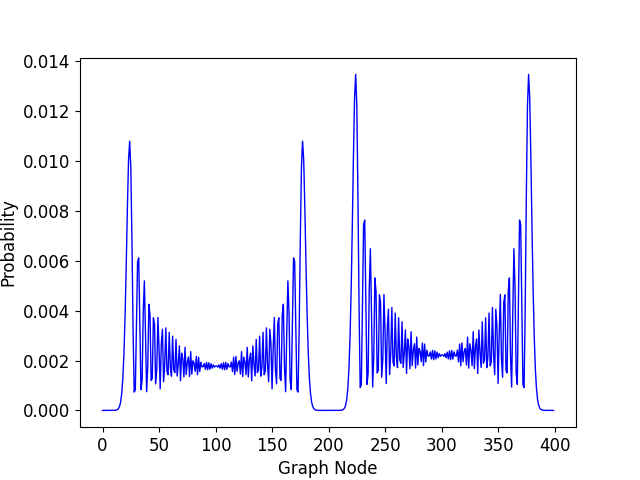
\includegraphics[scale=0.50]{img/QWAK/probDistCircLadder.png}
    \caption{Probability distribution for the continuous-time quantum walk on a circular ladder graph of size $N=400$, at $t=40$, with initial condition $\ket{\psi(0)}=\frac{\ket{100}+\ket{101}}{\sqrt{2}}$ and $\gamma=1$.} 
    \label{fig:probDistCircLadder}
\end{figure}
Here, we plot the distribution of a circular ladder graph built from the
Cartesian product of two cycle graphs, which explains the two separate
waveforms. Note that the \texttt{NetworkX} function builds two cycles with size
$n$, meaning our total number of nodes should be $2n$. This is accounted for
when initializing \texttt{State} and \texttt{Operator} objects by simply
defining their dimensions as a function of the \texttt{Graph} object. The
example also shows how to use the \texttt{customStateList} parameter, which
will raise an exception if the sum of the amplitudes is not $1$.\par

During initialization, the \texttt{QWAK} object uses the given parameters to
create attributes by calling the previously defined classes. After this, the
walk is evolved through the \texttt{runWalk} method: 
\begin{lstlisting}[style=commands,mathescape,language=Python]
    def runWalk(
            self, time: float = 0, initStateList: list = None, 
            customStateList: list = None) 
\end{lstlisting}
This method conforms previously defined build methods and catching any
exception thrown by them. The user may again choose to change initialization
values via the optional parameters. The \texttt{QWAK} class also offers all
previously mentioned methods for transport property analysis, as well as means
of accessing the individual building blocks of the quantum walk.  Further
examples, including transport property calculation and the stochastic quantum
walk simulation can be found in the \texttt{GitHub} repository. 

\end{document}
